\documentclass{article}
\usepackage[utf8]{inputenc}
\usepackage{hyperref}
\usepackage{graphicx}
\usepackage{subcaption}
\usepackage{cite}
\usepackage{float}
\usepackage{etoc}
\usepackage{blindtext}


%quote
\usepackage{epigraph}
\setlength\epigraphwidth{0.505\textwidth}
\setlength\epigraphrule{0pt}

% margins
\usepackage[a4paper, total={6in, 10in}]{geometry}

% spacing
\setlength{\parindent}{0em}
\setlength{\parskip}{1em}

% fonts (the same as NIPS 2016)
\renewcommand{\rmdefault}{ptm}
\renewcommand{\sfdefault}{phv}

\title{Komponenty obchodní logiky EJB\vspace{-1em}}
\author{Tomáš Vlk (vlktoma5@fit.cvut.cz)}
\date{\today}

\begin{document}

\maketitle

\section*{Úvod}

Enterprise Java Beans 3\footnote{EJB3} jsou řízené, serverové komponenty umožňující modulární tvorbu podnikových aplikací. Specifikace EJB3 je součástí množiny aplikačního programového rozhraní\footnote{API} definující Java Enterprise Edition.\par

Hlavním cílem EJB je oddělit je oddělit business logiku aplikace od prezentační\footnote{Například JSP} a persistentní vrstvy\footnote{Persistentní vrstva zajišťuje CRUD operace.}, ale také zajistit předpoklady pro integraci s ostatními technologiemi\footnote{Například JMS, JNDI a CORBA}.

\section*{Session Beans}

\subsection*{Stateless session beans}

Bezstavové beany neuchovávají stav relevantní pro klienta mezi obsluhou jeho jednotlivých požadavků. Pro obsloužení každého požadavku klienta je mu vždy na serveru přidělena samostatná instance, která je vyhrazena pouze tomuto klientovi v rámci jednoho daného požadavku. Důsledkem tohoto chování je thread safety.\par

Většinou se uchovávají v poolu ze kterého jsou odebrány na vykonání požadavku a poté jsou zase vráceny zpět. Nutná anotace jako \textbf{@Stateless}.\par

Při tvorbě instance beanu je možná injekce případných referencí a také možnost volat metodu \textbf{@PostConstruct}, která může zprostředkovat věci nutné k fungování beany\footnote{Například otevření přístupu do databáze}. Opakem metody \textbf{@PostConstruct} je metoda \textbf{@PreDestroy}, která se volá před smazáním beany. Vpřípadě systémové vyjímky se metoda \textbf{@PreDestroy} nevolá.

\begin{figure}[H]
\begin{center}
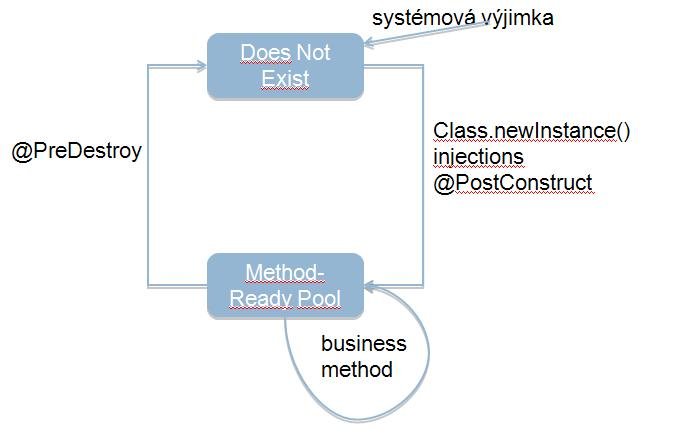
\includegraphics[scale=0.5]{Stateless_ejb.jpg}
\caption{Životní cyklus stateless beanu}
\end{center}
\end{figure}

\subsection*{Stateful session bean}

Jsou schopné uchovat svůj stav v rámci jedné session mezi jednotlivými voláními klienta. Každý klient má tedy vlastní instanci, která odpovídá pouze jemu a uchovává informace z předchozích interakcí. Může být ve stavu pasivace\footnote{Uložen pomocí perzistentní vrstvy}, pokud je nutné uvolnit paměť na serveru.\par

Musí být anotována pomocí \textbf{@Stateful}. Tvorba a odstraňování beanu probíhá stejně jako u stateless verze. Jediným rozdílem je pasivace, kdy bude zavolána metoda \textbf{@PrePasivate} před pasivací a následně metoda \textbf{@PostActivate} po opětovném obnovení beanu. Je zde také možnost nastavit beanu timeout po kterém bude automaticky odstraněn.

\begin{figure}[H]
\begin{center}
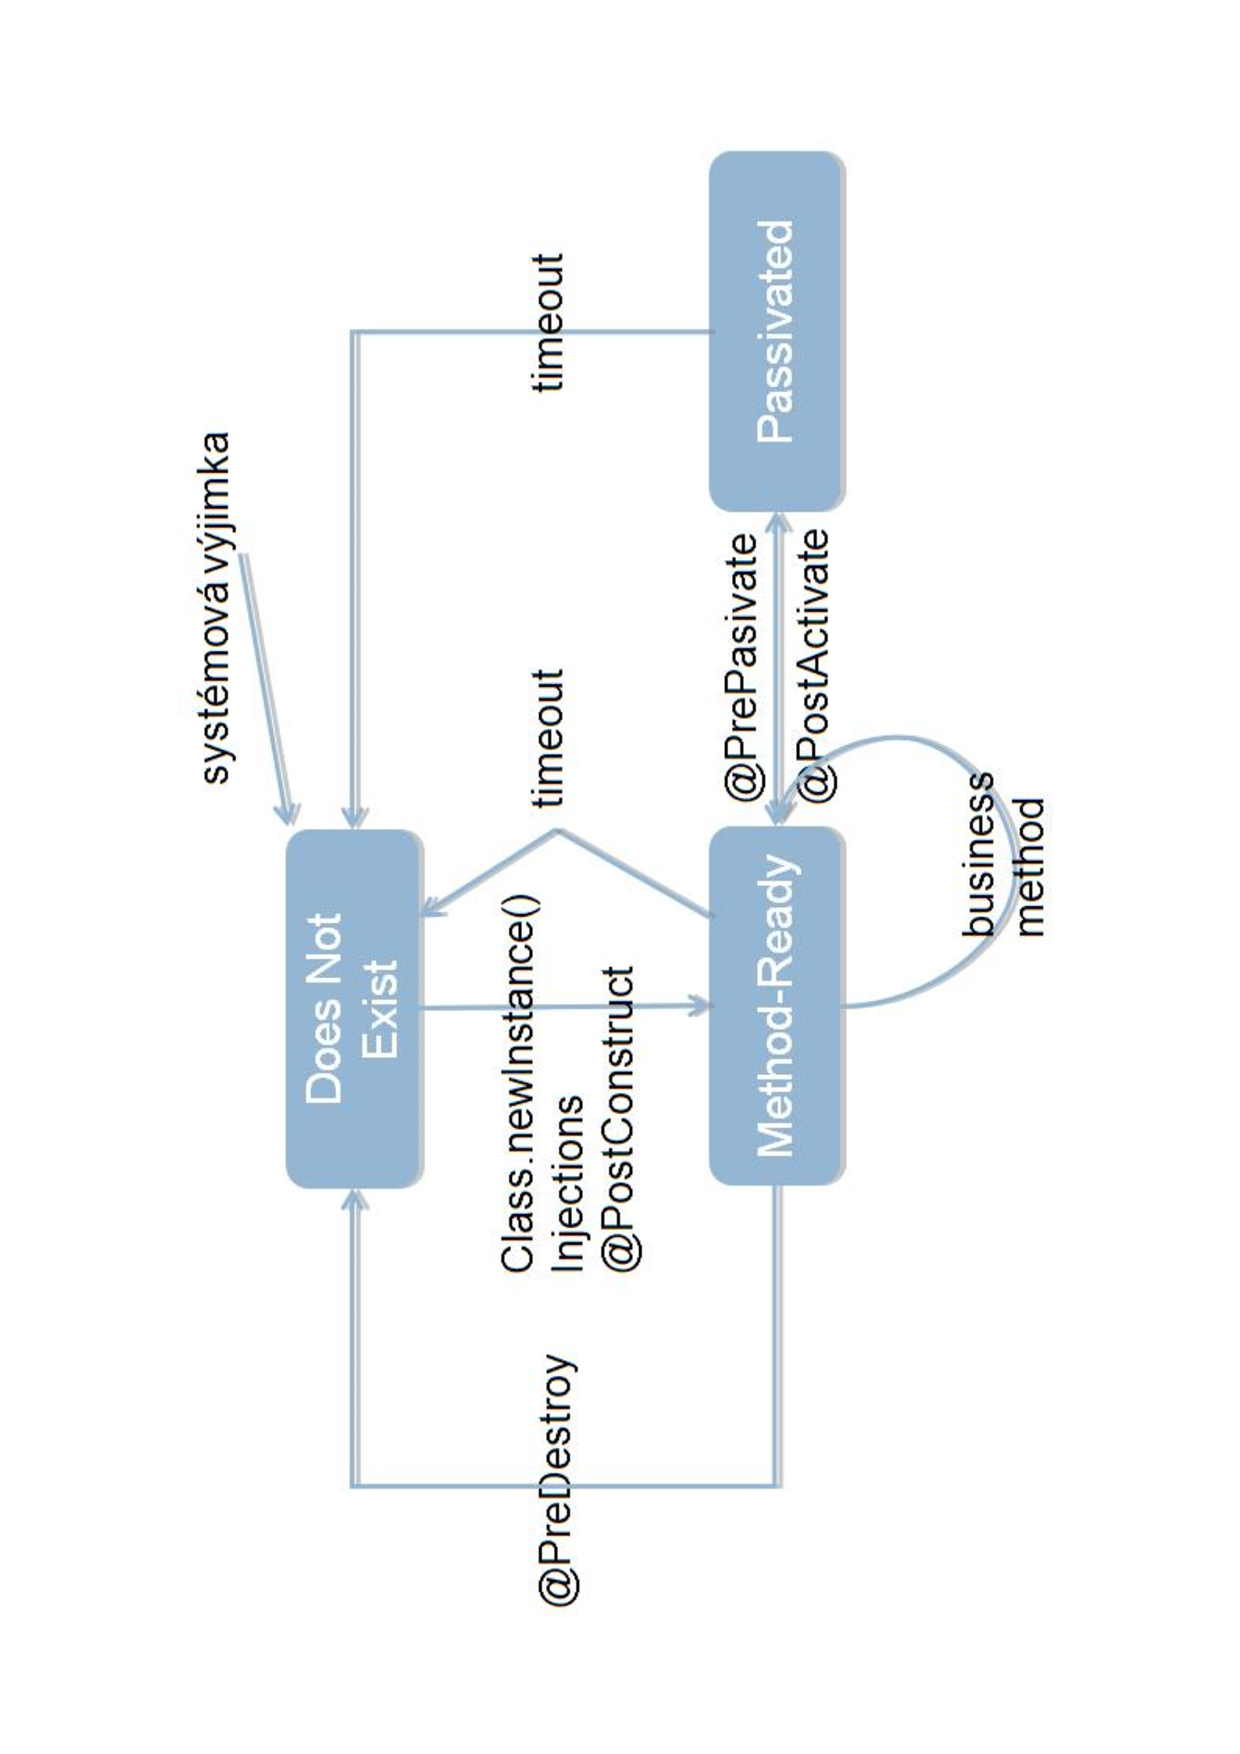
\includegraphics[scale=0.5, angle=270]{Stateful_ejb.pdf}
\caption{Životní cyklus statefull beanu}
\end{center}
\end{figure}

\subsection*{Singleton session bean}

Objekty s globálně sdíleným stavem. Přístup je řízen buď kontejnerem, nebo samotným beanem pomocí anotace \textbf{@Lock} a parametrem pro zámku pro čtení nebo zápis při volání metod. Anotace \textbf{@Startup} umožnuje vznik singletonu už při vzniku EJB kontejneru\footnote{Vhodné pro načítaní statických hodnot.}. Singleton je nutné anotovat jako \textbf{@Singleton}.

\section*{Message Driven Beans}

Beany řízené zprávami, jsou asynchroní, tudíž se používají k operacím, které nevyžadují okamžitou odpověď. Umožnují událostně řízené zpracování uvnitř EJB kontejneru.

\section*{EJB kontejner}

Dedikovaný virtuální prostor v aplikačním serveru pro EJB komponenty. Hlavní problematika řešená pomocí EJB kontejneru je:

\begin{itemize}
\item \textbf{Komunikace se vzdáleným klientem} - zjednodušuje komunikaci mezi klientem a aplikací
\item \textbf{Dependency injection} - zajišťuje naplnění deklarovaných proměnných\footnote{Například dalšími EJBeany, JMS, datovými zdroji, atd.}
\item \textbf{Řízení stavu} - kontejner udržuje v paměti stavy jednotlivých stavových (stateful) beanů a tím i vzdálený stav u klienta, kterému se jeví stav jakoby uložen lokálně
\item \textbf{Pooling} - vytváření poolu instancí pro bezstavové beany a message-driven beany
\item \textbf{Řízení životního cyklu} - stará se o vytváření, inicializaci a destrukci instancí beanů a další události
\item \textbf{Messaging} - umožňuje MDB poslouchat na JMS destinacích a konzumovat zprávy a zároveň odstiňuje programátora od komplikovaného API Java Messaging Service
\item \textbf{Management transakcí} - beany deklarují transakční vlastnosti metod, kontejner řeší commit a rollback
\item \textbf{Bezpečnost} - deklarace přístupů na úrovni tříd a metod
\item \textbf{Podpora souběžného zpracování} - vývojář nemusí řešit problémy synchronizace souběžných přístupů ke sdíleným datům
\item \textbf{Správa interceptorů} - komponenty umožňující odchytávat okamžik před a po volání metody
\item \textbf{Asynchronní volání metod}
\end{itemize}

\section*{Rozhraní}

Rozhraní slouží pro definování metod, které bude muset bean implementovat a poskytovat navenek pro manipulaci s jeho datovými atributy. Každý EJB musí implementovat aspoň jedno z níže uvedených rozhraní:

\begin{itemize}
\item \textbf{Lokální rozhraní} - pokud není žádné rozhraní u třídy definováno, má se za to, že bean je lokálního typu, což v praxi znamená, že běží a jeho metody jsou volány pouze v rámci jednoho Java Virtual Machine. Anotuje se jako @Local.
\item \textbf{Vzdálené rozhraní} - značeno anotací @Remote. Používá se při volání metod takovéhoto EJB z jiného vzdáleného JVM. K volání metod slouží distribuovaný protokol. Tímto způsobem lze vytvářet plnohodnotné klientské aplikace, které nejsou vázané pouze na webový prohlížeč.
\item \textbf{Endpoint rozhraní} - slouží k označení rozhraní přístupného pro webové služby. Anotováno @javax.jws.WebService.
\item \textbf{Message rozhraní} - implementováno Message Driven Beany. Rozhraní MD beanu je voláno Java Message Službou, když je doručena nová zpráva do fronty obsluhována nějekým Message-oriented-middlewarem.
\end{itemize}

\section*{Embedded kontejner}

Nabízí možnost spouštět EJB aplikace v prostředí Java SE.

\section*{Injektování EJB}

Do EJB můžeme injectovat další EJB. Dochází k tomu při vytvoření beany, to je zajištěno pomocí EJB kontejneru. Anotace \textbf{@EJB} se používá pro injektování jiné beany, a anotace \textbf{@Resource} pro injektování zdrojů dat nebo kontextu.

\end{document}
